\ifdefined\standalone 
\documentclass[12pt]{article}
\usepackage{graphicx}
\usepackage{float}
\usepackage[a4paper, margin=1in]{geometry}
\usepackage[utf8]{inputenc}
\usepackage{textcomp}
\usepackage{amsmath}
\usepackage{booktabs}
\usepackage{tikz}
\usepackage{enumitem}
\usetikzlibrary{decorations.pathmorphing,patterns}
\usepackage[hidelinks]{hyperref}
\usepackage[toc,page]{appendix}


\begin{document}
\fi

\section{Darcy Flow with Fixed Flux Boundary Conditions}

This verification case examines the behaviour of the pressure solver in a porous material under steady one-dimensional gas flow with an imposed gas mass flux.  
A uniform porous layer of thickness $L = 10~\mathrm{cm}$ is considered (Figure~\ref{fig:configuration_darcy_mfixed}).  
The temperature is fixed at $T_0 = 300~\mathrm{K}$, and the permeability of the material is $\bar{K} = 5\cdot 10^{-10} \; \mathrm{m^{2}}$. The background gas, gas properties and transport parameter are treated exactly as in Section \ref{Darcy_pfixed}.

At the top boundary, the pressure is imposed at $1~\mathrm{bar}$,while at the bottom boundary a mass flux is imposed:
\[
\dot{m}''(L) = 10~\mathrm{kg \cdot m^{-2} \cdot s^{-1}}.
\]



As shown in ~\ref{ann:analytical_pressure2}, the analytical pressure profile is:
\begin{equation}
P(z) = \sqrt{
P_0^2 + 2 \frac{\alpha}{\bar{K}} \dot{m}''_{\!L} \, z }.
\end{equation}

The mass flux is spatially uniform and equal to the imposed boundary value:
\begin{equation}
\dot{m}'' = \dot{m}''_{\!L} = 10~\mathrm{kg\cdot m^{-2}\cdot s^{-1}}.
\end{equation}

Figures~\ref{fig:viscosity_darcy_mfixed}, \ref{fig:pressure_darcy_mfixed}, and \ref{fig:flux_darcy_mfixed} present respectively the pressure distribution, the kinematic viscosity profile, and the mass flux comparison between the analytical solution and the Gpyro simulation.


\begin{figure}[H]
\centering

\begin{minipage}[t]{0.45\textwidth}
\centering
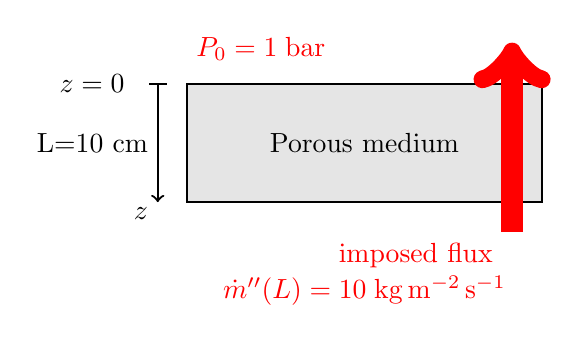
\begin{tikzpicture}[scale=0.75]

\draw[fill=gray!20,thick] (0,0) rectangle (6,2);
\node at (3,1) {Porous medium};

\draw[thick] (-0.35,2) -- (-0.65,2); 
\node[left] at (-0.9,2) {$z=0$};

\draw[thick,->] (-0.5,2) -- (-0.5,0);
\node[left] at (-0.5,1) {L=10~cm};
\node[left] at (-0.5,-0.2) {$z$};

\node[red, left] at (2.5,2.6) {$P_0= 1 \;\mathrm{bar}$};

\draw[red,line width=8pt,->] (5.5,-0.5) -- (5.5,2.7);
\node[red,anchor=west] at (2.4,-0.9)
    {imposed flux};
\node[red] at (3,-1.5) {$\dot{m}''(L)=10\;\mathrm{kg\,m^{-2}\,s^{-1}}$};

\end{tikzpicture}

\caption{Configuration schematic.}
\label{fig:configuration_darcy_mfixed}
\end{minipage}
\hfill
\begin{minipage}[t]{0.48\textwidth}
\centering
\includegraphics[width=\textwidth]{Pressure_darcy_mfixed.png}
\caption{Pressure profile along the porous domain.}
\label{fig:pressure_darcy_mfixed}
\end{minipage}

\end{figure}



\begin{figure}[H]
\centering
\begin{minipage}{0.48\textwidth}
\centering
\includegraphics[width=\textwidth]{Viscosity_darcy_mfixed.png}
\caption{Kinematic viscosity profile.}
\label{fig:viscosity_darcy_mfixed}
\end{minipage}
\hfill
\begin{minipage}{0.48\textwidth}
\centering
\includegraphics[width=\textwidth]{flux_darcy_mfixed.png}
\caption{Mass flux along the domain.}
\label{fig:flux_darcy_mfixed}
\end{minipage}
\end{figure}


\ifdefined\standalone
\end{document}
\fi



